\documentclass{article}\usepackage[]{graphicx}\usepackage[]{color}
%% maxwidth is the original width if it is less than linewidth
%% otherwise use linewidth (to make sure the graphics do not exceed the margin)
\makeatletter
\def\maxwidth{ %
  \ifdim\Gin@nat@width>\linewidth
    \linewidth
  \else
    \Gin@nat@width
  \fi
}
\makeatother

\definecolor{fgcolor}{rgb}{0.345, 0.345, 0.345}
\newcommand{\hlnum}[1]{\textcolor[rgb]{0.686,0.059,0.569}{#1}}%
\newcommand{\hlstr}[1]{\textcolor[rgb]{0.192,0.494,0.8}{#1}}%
\newcommand{\hlcom}[1]{\textcolor[rgb]{0.678,0.584,0.686}{\textit{#1}}}%
\newcommand{\hlopt}[1]{\textcolor[rgb]{0,0,0}{#1}}%
\newcommand{\hlstd}[1]{\textcolor[rgb]{0.345,0.345,0.345}{#1}}%
\newcommand{\hlkwa}[1]{\textcolor[rgb]{0.161,0.373,0.58}{\textbf{#1}}}%
\newcommand{\hlkwb}[1]{\textcolor[rgb]{0.69,0.353,0.396}{#1}}%
\newcommand{\hlkwc}[1]{\textcolor[rgb]{0.333,0.667,0.333}{#1}}%
\newcommand{\hlkwd}[1]{\textcolor[rgb]{0.737,0.353,0.396}{\textbf{#1}}}%

\usepackage{framed}
\makeatletter
\newenvironment{kframe}{%
 \def\at@end@of@kframe{}%
 \ifinner\ifhmode%
  \def\at@end@of@kframe{\end{minipage}}%
  \begin{minipage}{\columnwidth}%
 \fi\fi%
 \def\FrameCommand##1{\hskip\@totalleftmargin \hskip-\fboxsep
 \colorbox{shadecolor}{##1}\hskip-\fboxsep
     % There is no \\@totalrightmargin, so:
     \hskip-\linewidth \hskip-\@totalleftmargin \hskip\columnwidth}%
 \MakeFramed {\advance\hsize-\width
   \@totalleftmargin\z@ \linewidth\hsize
   \@setminipage}}%
 {\par\unskip\endMakeFramed%
 \at@end@of@kframe}
\makeatother

\definecolor{shadecolor}{rgb}{.97, .97, .97}
\definecolor{messagecolor}{rgb}{0, 0, 0}
\definecolor{warningcolor}{rgb}{1, 0, 1}
\definecolor{errorcolor}{rgb}{1, 0, 0}
\newenvironment{knitrout}{}{} % an empty environment to be redefined in TeX

\usepackage{alltt}

\usepackage{fancyhdr} % Required for custom headers
\usepackage{lastpage} % Required to determine the last page for the footer
\usepackage{extramarks} % Required for headers and footers
\usepackage{graphicx} % Required to insert images
\usepackage{hyperref}
\usepackage{amsmath} %for binomial pdf
\usepackage{parskip} % so that there's space bw paragraphs
\usepackage{float}
\usepackage{amsfonts}
\usepackage{hanging}
\usepackage{undertilde}
\usepackage{amssymb}


% Margins
\topmargin=-0.45in
\evensidemargin=0in
\oddsidemargin=0in
\textwidth=6.5in
\textheight=9.0in
\headsep=0.25in 

\linespread{1.1} % Line spacing

% Set up the header and footer
\pagestyle{fancy}
\lhead{STAT 532: Bayes} % Top left header
\chead{HW 6} % Top center header
\rhead{Andrea Mack} % Top right header
\lfoot{11/09/2016} % Bottom left footer
\cfoot{} % Bottom center footer
\rfoot{Page\ \thepage\ of\ \pageref{LastPage}} % Bottom right footer
\renewcommand\headrulewidth{0.4pt} % Size of the header rule
\renewcommand\footrulewidth{0.4pt} % Size of the footer rule

\setlength\parindent{0pt} % Removes all indentation from paragraphs
\setlength\parskip{0.5cm}
\restylefloat{table}

%----------------------------------------------------------------------------------------
%	DOCUMENT STRUCTURE COMMANDS
%	Skip this unless you know what you're doing
%----------------------------------------------------------------------------------------

% Header and footer for when a page split occurs within a problem environment
\newcommand{\enterProblemHeader}[1]{
\nobreak\extramarks{#1}{#1 continued on next page\ldots}\nobreak
\nobreak\extramarks{#1 (continued)}{#1 continued on next page\ldots}\nobreak
}

% Header and footer for when a page split occurs between problem environments
\newcommand{\exitProblemHeader}[1]{
\nobreak\extramarks{#1 (continued)}{#1 continued on next page\ldots}\nobreak
\nobreak\extramarks{#1}{}\nobreak
}


%----------------------------------------------------------------------------------------%
\IfFileExists{upquote.sty}{\usepackage{upquote}}{}
\begin{document}


\begin{enumerate}
\item%1 
{\it Stein's Paradox: Do not do.}


\item %2
{\it Derivation, see attached.}

\item%3
{\it (30 points) Generate data from a two-dimensional hierarchical normal model (e.g. students
within a school). Write code for a Gibbs sampler and convince me that your code returns the
correct answer.}

2D means two levels. The plots below will hopefully convince you my code worked because the true values are all within the posterior distributions and I used a weakly informative prior, so the priors should not affect the posteriors as much as the simulated data, which were simulated from the true process.

\begin{knitrout}
\definecolor{shadecolor}{rgb}{0.969, 0.969, 0.969}\color{fgcolor}
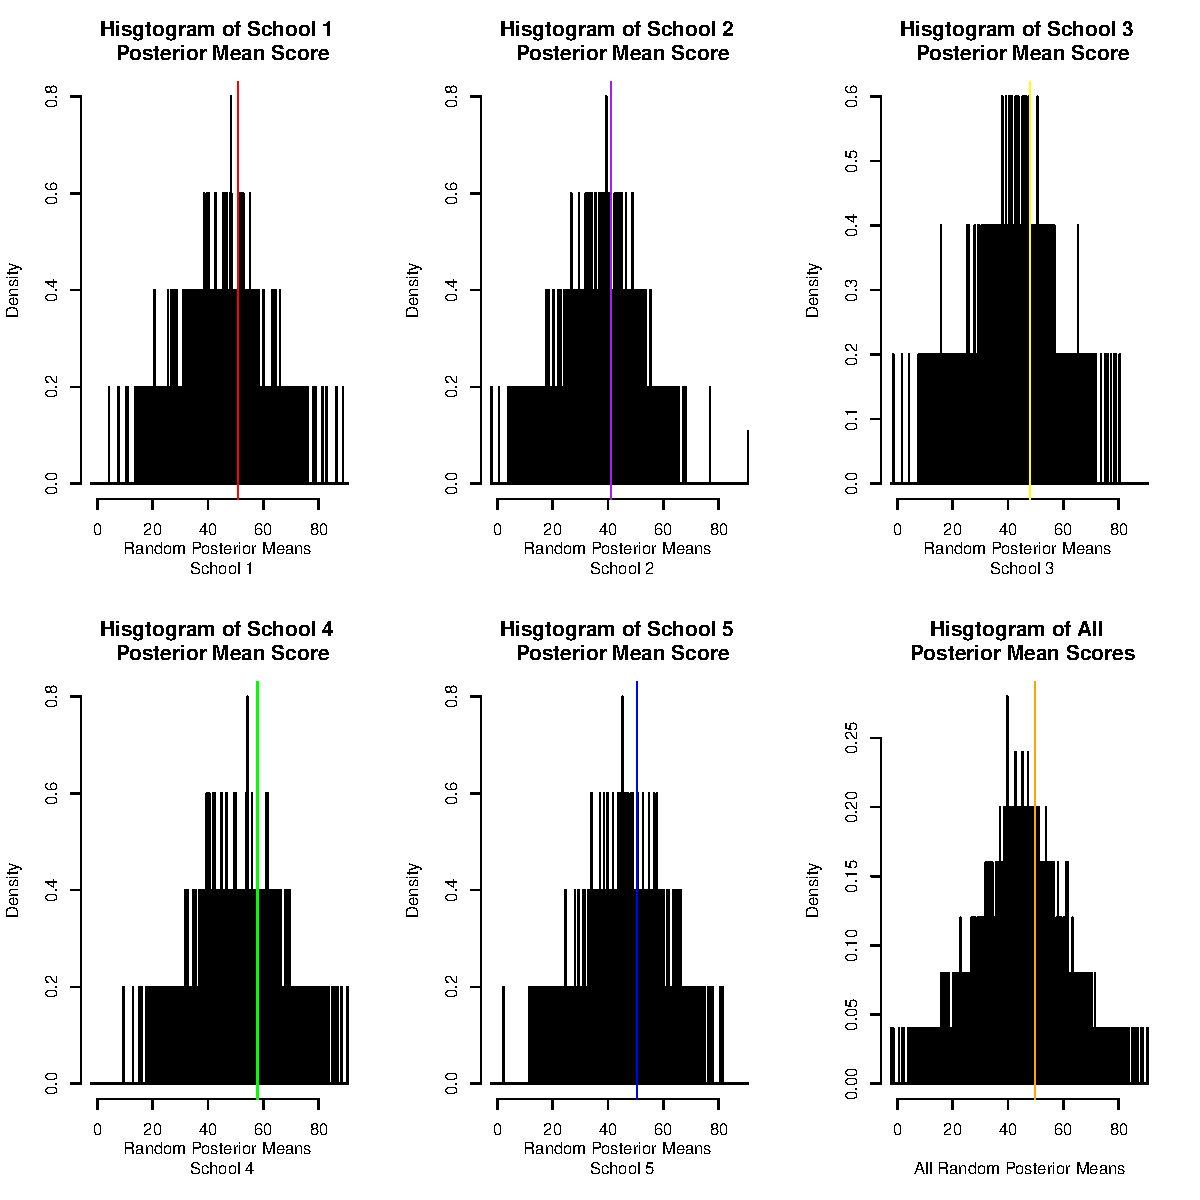
\includegraphics[width=\maxwidth]{figure/prob3-1} 

\end{knitrout}


\item%4
{\it Show that p($H_{o} | Data )$ = ($ 1 + \frac{1-\pi_{o}}{\pi_{o}}BF^{-1}$).}

p($H_{o} | Data ) = p(H_{o} | \utilde{x}$) = ($ 1 + \frac{1-\pi_{o}}{\pi_{o}}BF^{-1})^{-1}$

= ($ 1 + \frac{(1-\pi_{o})p(H_{1}|\utilde{x})p(H_{o})}{\pi_{o}P(H_{o}|\utilde{x})p(H_{1})})^{-1}$

= ($ 1 + \frac{(p(H_{1})p(H_{1}|\utilde{x})p(H_{o})}{p(H_{o})p(H_{o}|\utilde{x})p(H_{1})})^{-1}$

\rightarrow

$p(H_{o} | \utilde{x}) = p(H_{o}|\utilde{x})[p(H_{o}|\utilde_{x}) + p(H_{1}|\utilde_{x})]^{-1}$

\rightarrow

1 = 1 since $[p(H_{o}|\utilde_{x}) + p(H_{1}|\utilde_{x})] = 1 \QED$


\item%5
{\it (10 points) Summarize the paper you have selected for the final project. What about this
paper/method to you still not understand (be specific!)?}
\end{enumerate}

\begin{hangparas}{.25in}{1}
Diggle, P., & Lophaven, S. (2006). Bayesian geostatistical design. Scandinavian Journal of Statistics, 33(1), 53-64.
\end{hangparas}

Given a pre-existing sampling design, future studies may require fewer or more sampling points. Criteria for such called retrospective and prospective designs, respectively, reward accuracy in spatial prediction while accounting for parameter estimation. The authors' Bayesian design criteria approach, the spatial average of Var{S(x)|y}, and then compared to other developed criteria, ``classical". Comparisons between whether $\nu^2$ is known or unknown minimally affected the criteria. Under a prospective lattice design, close pairs is favored to in-fill added designs, but changes in locations of added points within the respective designs resulted in small changes in the criteria.


{\bf Still not understood:}
\begin{itemize}
\item {\it p. 54 line 2:} What is meant by ``proper allowance" exactly?

\item {\it p. 56 equation (1):} Why do they have to integrate out $\theta$ to make predictions? Is [$s|Y,\theta$] not sufficient?

\item In general, I don't understand the exact model fit to point reference data. Also, the authors say they assumed an exponential correlation function on p. 57, and I don't know how that was done, in a classical or bayesian framework. 

\item {\it bottom of p. 57:} In general, what about classical design criteria results in ``well separated" monitoring sites compared to the Bayesian approach?

\item {\it p. 61:} What are the implications of the locations of the added points not affecting the criteria much as the way the added points entered? Also, why did the authors do the 5 replicates?

\item {\bf Other terms/notation:}
\begin{itemize}
\item kringing

\item stoichasitc process

\item Notation p. 56, how does [S$|$Y] differ from [T$|$Y], T = target, so is this like popuation (target) and sample (observed)?

\item Method in Diggle et al. (2003) to generate direct Monte Carlo samples

\item Where does the noise-to-signal variance ratio come in?

\item Eutrophication

\item Exact definition of diffuse prior, I assume it's flat but not improper, but will look this up.

\end{itemize}
\end{itemize}

\section*{R Code}
\begin{enumerate}
\setcounter{enumi}{3}
{\tiny
\item 
\begin{knitrout}
\definecolor{shadecolor}{rgb}{0.969, 0.969, 0.969}\color{fgcolor}\begin{kframe}
\begin{alltt}
\hlstd{Y.school.mathscore}\hlkwb{<-}\hlkwd{dget}\hlstd{(}\hlstr{"https://www.stat.washington.edu/~pdhoff/Book/Data/data/Y.school.mathscore"}\hlstd{)}

 \hlstd{Y} \hlkwb{<-} \hlstd{Y.school.mathscore}
 \hlcom{#head(Y)}

 \hlcom{### say there are 5 schools with 12 classes in each school,}
 \hlcom{### say elementary schools in a town the size of bozeman}

 \hlstd{Z} \hlkwb{<-} \hlkwa{NULL}
 \hlstd{Z}\hlopt{$}\hlstd{school} \hlkwb{<-} \hlkwd{c}\hlstd{(}\hlkwd{rep}\hlstd{(}\hlnum{1}\hlstd{,}\hlnum{12}\hlstd{),} \hlkwd{rep}\hlstd{(}\hlnum{2}\hlstd{,}\hlnum{12}\hlstd{),} \hlkwd{rep}\hlstd{(}\hlnum{3}\hlstd{,}\hlnum{12}\hlstd{),} \hlkwd{rep}\hlstd{(}\hlnum{4}\hlstd{,}\hlnum{12}\hlstd{),} \hlkwd{rep}\hlstd{(}\hlnum{5}\hlstd{,}\hlnum{12}\hlstd{))}

 \hlcom{### there are two classes of each k-5 grades, lets say all teachers within a}
 \hlcom{### grade level produce the same quality of students}

 \hlcom{### to make things interesting, set school means to first five of the hoff data set}

 \hlstd{true.thetaj} \hlkwb{<-} \hlkwd{by}\hlstd{(Y[,}\hlnum{2}\hlstd{],} \hlkwd{as.factor}\hlstd{(}\hlkwd{as.character}\hlstd{(Y[,}\hlnum{1}\hlstd{])), mean)[}\hlnum{1}\hlopt{:}\hlnum{5}\hlstd{]}

 \hlcom{### simplify things, each school has the same variability, use the variation from all schools in hoff}

 \hlstd{true.sigma2} \hlkwb{<-} \hlkwd{var}\hlstd{(Y[,}\hlnum{2}\hlstd{])}

 \hlcom{### make class data from school data}
 \hlkwd{set.seed}\hlstd{(}\hlnum{53206}\hlstd{)}
 \hlstd{a1} \hlkwb{<-} \hlkwd{rnorm}\hlstd{(}\hlnum{12}\hlstd{,true.thetaj[}\hlnum{1}\hlstd{],} \hlkwc{sd} \hlstd{=} \hlkwd{sqrt}\hlstd{(true.sigma2))}
 \hlstd{a2} \hlkwb{<-} \hlkwd{rnorm}\hlstd{(}\hlnum{12}\hlstd{,true.thetaj[}\hlnum{2}\hlstd{],} \hlkwc{sd} \hlstd{=} \hlkwd{sqrt}\hlstd{(true.sigma2))}
 \hlstd{a3} \hlkwb{<-} \hlkwd{rnorm}\hlstd{(}\hlnum{12}\hlstd{,true.thetaj[}\hlnum{3}\hlstd{],} \hlkwc{sd} \hlstd{=} \hlkwd{sqrt}\hlstd{(true.sigma2))}
 \hlstd{a4} \hlkwb{<-} \hlkwd{rnorm}\hlstd{(}\hlnum{12}\hlstd{,true.thetaj[}\hlnum{4}\hlstd{],} \hlkwc{sd} \hlstd{=} \hlkwd{sqrt}\hlstd{(true.sigma2))}
 \hlstd{a5} \hlkwb{<-} \hlkwd{rnorm}\hlstd{(}\hlnum{12}\hlstd{,true.thetaj[}\hlnum{5}\hlstd{],} \hlkwc{sd} \hlstd{=} \hlkwd{sqrt}\hlstd{(true.sigma2))}

 \hlstd{Z}\hlopt{$}\hlstd{mathscore} \hlkwb{<-} \hlkwd{c}\hlstd{(a1,a2,a3,a4,a5)}

 \hlstd{Y} \hlkwb{<-} \hlkwd{data.frame}\hlstd{(Z)}

 \hlcom{### weakly informative priors}

 \hlcom{#prior on sigma2}
 \hlstd{nu.0}\hlkwb{<-}\hlnum{1}
 \hlstd{sigmasq.0}\hlkwb{<-}\hlnum{100}

 \hlcom{#prior on tau2, uses same sigmasq.0 from prior on sigma2, but here it is called tausq.0}
 \hlstd{eta.0}\hlkwb{<-}\hlnum{1}
 \hlstd{tausq.0}\hlkwb{<-}\hlnum{100}

 \hlcom{#prior on mu = mean of group math scores, don't have any intuition about these}
 \hlcom{#prior mean is 50, set prior variance to 144 say}

 \hlstd{mu.0}\hlkwb{<-}\hlnum{0}
 \hlstd{gammasq.0}\hlkwb{<-}\hlnum{144}
 \hlcom{###}

 \hlcom{### starting values}

 \hlstd{m} \hlkwb{<-} \hlnum{5} \hlcom{# number of schools}

 \hlcom{#find the mean, variance, and sample size of each school}
 \hlstd{n}\hlkwb{<-}\hlstd{sv}\hlkwb{<-}\hlstd{ybar}\hlkwb{<-}\hlkwd{rep}\hlstd{(}\hlnum{NA}\hlstd{,m)}
 \hlkwa{for}\hlstd{(j} \hlkwa{in} \hlnum{1}\hlopt{:}\hlstd{m)}
 \hlstd{\{}
   \hlcom{#mean by group}
 \hlstd{ybar[j]}\hlkwb{<-}\hlkwd{mean}\hlstd{(Y[Y[,}\hlnum{1}\hlstd{]}\hlopt{==}\hlstd{j,}\hlnum{2}\hlstd{])}
    \hlcom{#var by group}
 \hlstd{sv[j]}\hlkwb{<-}\hlkwd{var}\hlstd{(Y[Y[,}\hlnum{1}\hlstd{]}\hlopt{==}\hlstd{j,}\hlnum{2}\hlstd{])}
    \hlcom{#n by group}
 \hlstd{n[j]}\hlkwb{<-}\hlkwd{sum}\hlstd{(Y[,}\hlnum{1}\hlstd{]} \hlopt{==}\hlstd{j)}
 \hlstd{\}}
 \hlstd{theta}\hlkwb{<-}\hlstd{ybar}
 \hlcom{#sigma2 is the average group variance}
 \hlstd{sigma2}\hlkwb{<-}\hlkwd{mean}\hlstd{(sv)}
 \hlstd{mu}\hlkwb{<-}\hlkwd{mean}\hlstd{(theta)}
 \hlcom{#tau2 is the variance of the group means}
 \hlstd{tau2}\hlkwb{<-}\hlkwd{var}\hlstd{(theta)}
 \hlcom{###}

 \hlcom{### setup MCMC}
 \hlkwd{set.seed}\hlstd{(}\hlnum{5326}\hlstd{)}
 \hlstd{S}\hlkwb{<-}\hlnum{5000}
 \hlstd{THETA}\hlkwb{<-}\hlkwd{matrix}\hlstd{(} \hlkwc{nrow}\hlstd{=S,}\hlkwc{ncol}\hlstd{=m)}
 \hlstd{MST}\hlkwb{<-}\hlkwd{matrix}\hlstd{(} \hlkwc{nrow}\hlstd{=S,}\hlkwc{ncol}\hlstd{=}\hlnum{3}\hlstd{)}
 \hlcom{###}

 \hlcom{### MCMC algorithm}
 \hlkwa{for}\hlstd{(s} \hlkwa{in} \hlnum{1}\hlopt{:}\hlstd{S)}
 \hlstd{\{}

 \hlcom{# sample new values of the thetas}
 \hlkwa{for}\hlstd{(j} \hlkwa{in} \hlnum{1}\hlopt{:}\hlstd{m)}
 \hlstd{\{}
 \hlstd{vtheta}\hlkwb{<-}\hlnum{1}\hlopt{/}\hlstd{(n[j]}\hlopt{/}\hlstd{sigma2}\hlopt{+}\hlnum{1}\hlopt{/}\hlstd{tau2)}

 \hlstd{etheta}\hlkwb{<-}\hlstd{vtheta}\hlopt{*}\hlstd{(ybar[j]}\hlopt{*}\hlstd{n[j]}\hlopt{/}\hlstd{sigma2}\hlopt{+}\hlstd{mu}\hlopt{/}\hlstd{tau2)}
 \hlstd{theta[j]}\hlkwb{<-}\hlkwd{rnorm}\hlstd{(}\hlnum{1}\hlstd{,etheta,}\hlkwd{sqrt}\hlstd{(vtheta))}
 \hlstd{\}}
\hlcom{#\}}
 \hlcom{#sample new value of sigma2}
 \hlstd{nun}\hlkwb{<-}\hlstd{nu.0}\hlopt{+}\hlkwd{sum}\hlstd{(n)}
 \hlstd{ss}\hlkwb{<-}\hlstd{nu.0}\hlopt{*}\hlstd{sigmasq.0;}

 \hlstd{ss1} \hlkwb{<-} \hlstd{ss} \hlopt{+} \hlkwd{sum}\hlstd{((Y[}\hlnum{1}\hlopt{:}\hlnum{12}\hlstd{,}\hlnum{2}\hlstd{]} \hlopt{-} \hlstd{theta[}\hlnum{1}\hlstd{])}\hlopt{^}\hlnum{2}\hlstd{)}
 \hlstd{ss2} \hlkwb{<-} \hlstd{ss} \hlopt{+} \hlkwd{sum}\hlstd{((Y[}\hlnum{13}\hlopt{:}\hlnum{24}\hlstd{,}\hlnum{2}\hlstd{]} \hlopt{-} \hlstd{theta[}\hlnum{2}\hlstd{])}\hlopt{^}\hlnum{2}\hlstd{)}
 \hlstd{ss3} \hlkwb{<-} \hlstd{ss} \hlopt{+} \hlkwd{sum}\hlstd{((Y[}\hlnum{25}\hlopt{:}\hlnum{36}\hlstd{,}\hlnum{2}\hlstd{]} \hlopt{-} \hlstd{theta[}\hlnum{3}\hlstd{])}\hlopt{^}\hlnum{2}\hlstd{)}
 \hlstd{ss4} \hlkwb{<-} \hlstd{ss} \hlopt{+} \hlkwd{sum}\hlstd{((Y[}\hlnum{37}\hlopt{:}\hlnum{48}\hlstd{,}\hlnum{2}\hlstd{]} \hlopt{-} \hlstd{theta[}\hlnum{4}\hlstd{])}\hlopt{^}\hlnum{2}\hlstd{)}
 \hlstd{ss5} \hlkwb{<-} \hlstd{ss} \hlopt{+} \hlkwd{sum}\hlstd{((Y[}\hlnum{49}\hlopt{:}\hlnum{60}\hlstd{,}\hlnum{2}\hlstd{]} \hlopt{-} \hlstd{theta[}\hlnum{5}\hlstd{])}\hlopt{^}\hlnum{2}\hlstd{)}

 \hlstd{ssk} \hlkwb{<-} \hlkwd{c}\hlstd{(ss1,ss2,ss3,ss4,ss5)}

 \hlcom{#don't understand how the code below works}
 \hlkwa{for}\hlstd{(j} \hlkwa{in} \hlnum{1}\hlopt{:}\hlstd{m)\{}
 \hlstd{ss}\hlkwb{<-}\hlstd{ss}\hlopt{+}\hlkwd{sum}\hlstd{((Y[,}\hlnum{2}\hlstd{]}\hlopt{-}\hlstd{theta[j])}\hlopt{^}\hlnum{2}\hlstd{)}
 \hlstd{\}}

 \hlstd{sigma2}\hlkwb{<-}\hlnum{1}\hlopt{/}\hlkwd{rgamma}\hlstd{(}\hlnum{1}\hlstd{,nun}\hlopt{/}\hlnum{2}\hlstd{,ss}\hlopt{/}\hlnum{2}\hlstd{)}

 \hlcom{#sample a new value of mu}
 \hlstd{vmu}\hlkwb{<-} \hlnum{1}\hlopt{/}\hlstd{(m}\hlopt{/}\hlstd{tau2}\hlopt{+}\hlnum{1}\hlopt{/}\hlstd{gammasq.0)}
 \hlstd{emu}\hlkwb{<-} \hlstd{vmu}\hlopt{*}\hlstd{(m}\hlopt{*}\hlkwd{mean}\hlstd{(theta)}\hlopt{/}\hlstd{tau2} \hlopt{+} \hlstd{mu.0}\hlopt{/}\hlstd{gammasq.0)}
 \hlstd{mu}\hlkwb{<-}\hlkwd{rnorm}\hlstd{(}\hlnum{1}\hlstd{,emu,}\hlkwd{sqrt}\hlstd{(vmu))}

 \hlcom{# sample a new value of tau2}
 \hlstd{etam}\hlkwb{<-}\hlstd{eta.0}\hlopt{+}\hlstd{m}
 \hlstd{ss}\hlkwb{<-} \hlstd{eta.0}\hlopt{*}\hlstd{tausq.0} \hlopt{+} \hlkwd{sum}\hlstd{( (theta}\hlopt{-}\hlstd{mu)}\hlopt{^}\hlnum{2} \hlstd{)}
 \hlstd{tau2}\hlkwb{<-}\hlnum{1}\hlopt{/}\hlkwd{rgamma}\hlstd{(}\hlnum{1}\hlstd{,etam}\hlopt{/}\hlnum{2}\hlstd{,ss}\hlopt{/}\hlnum{2}\hlstd{)}

 \hlcom{#store results}
 \hlcom{#for(s in 1:S) \{}
 \hlstd{THETA[s,]}\hlkwb{<-}\hlstd{theta}
 \hlstd{MST[s,]}\hlkwb{<-}\hlkwd{c}\hlstd{(mu,sigma2,tau2)}
 \hlstd{\}}

 \hlkwd{par}\hlstd{(}\hlkwc{mfrow}\hlstd{=}\hlkwd{c}\hlstd{(}\hlnum{2}\hlstd{,}\hlnum{3}\hlstd{))}
 \hlkwd{hist}\hlstd{(THETA[,}\hlnum{1}\hlstd{],} \hlkwc{breaks} \hlstd{=} \hlkwd{c}\hlstd{(}\hlkwd{min}\hlstd{(THETA)} \hlopt{-} \hlnum{0.001}\hlstd{,} \hlkwd{seq}\hlstd{(}\hlkwd{min}\hlstd{(THETA),} \hlkwd{max}\hlstd{(THETA),}\hlkwc{by} \hlstd{=} \hlnum{0.001}\hlstd{),}
                            \hlkwd{max}\hlstd{(THETA)} \hlopt{+} \hlnum{0.001}\hlstd{),}
      \hlkwc{main} \hlstd{=} \hlstr{"Hisgtogram of School 1 \textbackslash{}n Posterior Mean Score"}\hlstd{,} \hlkwc{xlab} \hlstd{=}
        \hlstr{"Random Posterior Means \textbackslash{}n School 1"}\hlstd{)}
 \hlkwd{abline}\hlstd{(}\hlkwc{v}\hlstd{=true.thetaj[}\hlnum{1}\hlstd{],} \hlkwc{col} \hlstd{=} \hlstr{"red"}\hlstd{)}

 \hlkwd{hist}\hlstd{(THETA[,}\hlnum{2}\hlstd{],} \hlkwc{breaks} \hlstd{=} \hlkwd{c}\hlstd{(}\hlkwd{min}\hlstd{(THETA)} \hlopt{-} \hlnum{0.001}\hlstd{,} \hlkwd{seq}\hlstd{(}\hlkwd{min}\hlstd{(THETA),} \hlkwd{max}\hlstd{(THETA),}\hlkwc{by} \hlstd{=} \hlnum{0.001}\hlstd{),}
                            \hlkwd{max}\hlstd{(THETA)} \hlopt{+} \hlnum{0.001}\hlstd{),}
      \hlkwc{main} \hlstd{=} \hlstr{"Hisgtogram of School 2 \textbackslash{}n Posterior Mean Score"}\hlstd{,} \hlkwc{xlab} \hlstd{=}
        \hlstr{"Random Posterior Means \textbackslash{}n School 2"}\hlstd{)}
 \hlkwd{abline}\hlstd{(}\hlkwc{v}\hlstd{=true.thetaj[}\hlnum{2}\hlstd{],} \hlkwc{col} \hlstd{=} \hlstr{"purple"}\hlstd{)}

 \hlkwd{hist}\hlstd{(THETA[,}\hlnum{3}\hlstd{],} \hlkwc{breaks} \hlstd{=} \hlkwd{c}\hlstd{(}\hlkwd{min}\hlstd{(THETA)} \hlopt{-} \hlnum{0.001}\hlstd{,} \hlkwd{seq}\hlstd{(}\hlkwd{min}\hlstd{(THETA),} \hlkwd{max}\hlstd{(THETA),}\hlkwc{by} \hlstd{=} \hlnum{0.001}\hlstd{),}
                            \hlkwd{max}\hlstd{(THETA)} \hlopt{+} \hlnum{0.001}\hlstd{),}
      \hlkwc{main} \hlstd{=} \hlstr{"Hisgtogram of School 3 \textbackslash{}n Posterior Mean Score"}\hlstd{,} \hlkwc{xlab} \hlstd{=}
        \hlstr{"Random Posterior Means \textbackslash{}n School 3"}\hlstd{)}
  \hlkwd{abline}\hlstd{(}\hlkwc{v}\hlstd{=true.thetaj[}\hlnum{3}\hlstd{],} \hlkwc{col} \hlstd{=} \hlstr{"yellow"}\hlstd{)}

  \hlkwd{hist}\hlstd{(THETA[,}\hlnum{4}\hlstd{],} \hlkwc{breaks} \hlstd{=} \hlkwd{c}\hlstd{(}\hlkwd{min}\hlstd{(THETA)} \hlopt{-} \hlnum{0.001}\hlstd{,} \hlkwd{seq}\hlstd{(}\hlkwd{min}\hlstd{(THETA),} \hlkwd{max}\hlstd{(THETA),}\hlkwc{by} \hlstd{=} \hlnum{0.001}\hlstd{),}
                            \hlkwd{max}\hlstd{(THETA)} \hlopt{+} \hlnum{0.001}\hlstd{),}
      \hlkwc{main} \hlstd{=} \hlstr{"Hisgtogram of School 4 \textbackslash{}n Posterior Mean Score"}\hlstd{,} \hlkwc{xlab} \hlstd{=}
        \hlstr{"Random Posterior Means \textbackslash{}n School 4"}\hlstd{)}

 \hlkwd{abline}\hlstd{(}\hlkwc{v}\hlstd{=true.thetaj[}\hlnum{4}\hlstd{],} \hlkwc{col} \hlstd{=} \hlstr{"green"}\hlstd{)}

 \hlkwd{hist}\hlstd{(THETA[,}\hlnum{5}\hlstd{],} \hlkwc{breaks} \hlstd{=} \hlkwd{c}\hlstd{(}\hlkwd{min}\hlstd{(THETA)} \hlopt{-} \hlnum{0.001}\hlstd{,} \hlkwd{seq}\hlstd{(}\hlkwd{min}\hlstd{(THETA),} \hlkwd{max}\hlstd{(THETA),}\hlkwc{by} \hlstd{=} \hlnum{0.001}\hlstd{),}
                            \hlkwd{max}\hlstd{(THETA)} \hlopt{+} \hlnum{0.001}\hlstd{),}
      \hlkwc{main} \hlstd{=} \hlstr{"Hisgtogram of School 5 \textbackslash{}n Posterior Mean Score"}\hlstd{,} \hlkwc{xlab} \hlstd{=} \hlstr{"Random Posterior Means \textbackslash{}n School 5"}\hlstd{)}
  \hlkwd{abline}\hlstd{(}\hlkwc{v}\hlstd{=true.thetaj[}\hlnum{5}\hlstd{],} \hlkwc{col} \hlstd{=} \hlstr{"blue"}\hlstd{)}

  \hlkwd{hist}\hlstd{(THETA,} \hlkwc{breaks} \hlstd{=} \hlkwd{c}\hlstd{(}\hlkwd{min}\hlstd{(THETA)} \hlopt{-} \hlnum{0.001}\hlstd{,} \hlkwd{seq}\hlstd{(}\hlkwd{min}\hlstd{(THETA),} \hlkwd{max}\hlstd{(THETA),}\hlkwc{by} \hlstd{=} \hlnum{0.001}\hlstd{),}
                            \hlkwd{max}\hlstd{(THETA)} \hlopt{+} \hlnum{0.001}\hlstd{),}
      \hlkwc{main} \hlstd{=} \hlstr{"Hisgtogram of All \textbackslash{}n Posterior Mean Scores"}\hlstd{,} \hlkwc{xlab} \hlstd{=} \hlstr{"All Random Posterior Means"}\hlstd{)}
  \hlkwd{abline}\hlstd{(}\hlkwc{v}\hlstd{=}\hlkwd{mean}\hlstd{(true.thetaj),} \hlkwc{col} \hlstd{=} \hlstr{"orange"}\hlstd{)}
\end{alltt}
\end{kframe}
\end{knitrout}
}
\end{enumerate}

\end{document}
